\section{Auswertung}
\label{sec:auswertung}

%==========Nico=================
\subsection{Berechnung von $\overline{\Delta l_n}$}
\label{sub:auswertung->MittelwertResonanzabstand}
Die Tabellen \ref{tab:auswertung->MittelwertResonanzabstand->Messung1} bis \ref{tab:auswertung->MittelwertResonanzabstand->Messung4} zeigen unsere Messergebnisse mit den dazu gehörigen Differenzen. $\Delta l_n$ wurde wie folgt berechnet:
\begin{align}
	\Delta l_n &= l_{max,n} - l_{min,n}
\end{align}
\begin{tabelle}
	\caption{Messwerte mit berechneten Differenzen für die 1. Messung ($500~Hz$)}
	\label{tab:auswertung->MittelwertResonanzabstand->Messung1}
	\sisetup{round-precision=1}
	\begin{tabular}{|c|c|c|c|c|c|c|c|c|c|c|c|}
		\hline \rowcolor{firstcsvrow}
		Messung & 1 & 2 & 3 & 4 & 5 & 6 & 7 & 8 & 9 & 10 & Mittelwert \\
		\csvreader[separator=semicolon, late after line = \\\hline]{./tables/A1a.csv}{}{
			\csvcoli & $\num{\csvcolii}$ & $\num{\csvcoliii}$ & $\num{\csvcoliv}$ & $\num{\csvcolv}$ & $\num{\csvcolvi}$ & $\num{\csvcolvii}$ & $\num{\csvcolviii}$ & $\num{\csvcolix}$ & $\num{\csvcolx}$ & $\num{\csvcolxi}$ & $\num{\csvcolxii}$
		}
	\end{tabular}
\end{tabelle}
\begin{tabelle}
	\caption{Messwerte mit berechneten Differenzen für die 2. Messung ($1000~Hz$)}
	\label{tab:auswertung->MittelwertResonanzabstand->Messung2}
	\sisetup{round-precision=1}
	\begin{tabular}{|c|c|c|c|c|c|c|c|c|c|c|c|}
		\hline \rowcolor{firstcsvrow}
		Messung & 1 & 2 & 3 & 4 & 5 & 6 & 7 & 8 & 9 & 10 & Mittelwert \\
		\csvreader[separator=semicolon, late after line = \\\hline]{./tables/A1b.csv}{}{
			\csvcoli & $\num{\csvcolii}$ & $\num{\csvcoliii}$ & $\num{\csvcoliv}$ & $\num{\csvcolv}$ & $\num{\csvcolvi}$ & $\num{\csvcolvii}$ & $\num{\csvcolviii}$ & $\num{\csvcolix}$ & $\num{\csvcolx}$ & $\num{\csvcolxi}$ & $\num{\csvcolxii}$
		}
	\end{tabular}
\end{tabelle}
\begin{tabelle}
	\caption{Messwerte mit berechneten Differenzen für die 3. Messung ($1500~Hz$)}
	\label{tab:auswertung->MittelwertResonanzabstand->Messung3}
	\sisetup{round-precision=1}
	\begin{tabular}{|c|c|c|c|c|c|c|c|c|c|c|c|}
		\hline \rowcolor{firstcsvrow}
		Messung & 1 & 2 & 3 & 4 & 5 & 6 & 7 & 8 & 9 & 10 & Mittelwert \\
		\csvreader[separator=semicolon, late after line = \\\hline]{./tables/A1c.csv}{}{
			\csvcoli & $\num{\csvcolii}$ & $\num{\csvcoliii}$ & $\num{\csvcoliv}$ & $\num{\csvcolv}$ & $\num{\csvcolvi}$ & $\num{\csvcolvii}$ & $\num{\csvcolviii}$ & $\num{\csvcolix}$ & $\num{\csvcolx}$ & $\num{\csvcolxi}$ & $\num{\csvcolxii}$
		}
	\end{tabular}
\end{tabelle}
\begin{tabelle}
	\caption{Messwerte mit berechneten Differenzen für die 4. Messung ($2000~Hz$)}
	\label{tab:auswertung->MittelwertResonanzabstand->Messung4}
	\sisetup{round-precision=1}
	\begin{tabular}{|c|c|c|c|c|c|c|c|c|c|c|c|}
		\hline \rowcolor{firstcsvrow}
		Messung & 1 & 2 & 3 & 4 & 5 & 6 & 7 & 8 & 9 & 10 & Mittelwert \\
		\csvreader[separator=semicolon, late after line = \\\hline]{./tables/A1d.csv}{}{
			\csvcoli & $\num{\csvcolii}$ & $\num{\csvcoliii}$ & $\num{\csvcoliv}$ & $\num{\csvcolv}$ & $\num{\csvcolvi}$ & $\num{\csvcolvii}$ & $\num{\csvcolviii}$ & $\num{\csvcolix}$ & $\num{\csvcolx}$ & $\num{\csvcolxi}$ & $\num{\csvcolxii}$
		}
	\end{tabular}
\end{tabelle}

\subsection{Berechnung der Wellenlänge $\lambda$}
\label{sub:auswertung->Wellenlaenge}
Abbildung \ref{ab:auswertung->lambda->begruendung} zeigt die stehende Welle im Resonanzrohr mit den dazugehörigen Längenbeziehungen. Die Anzahl der Resonanzen ist in blau eingezeichnet, wobei bei der Resonanz $l_{min}$ mit eins zu zählen begonnen wurde.
\begin{abbildung}
	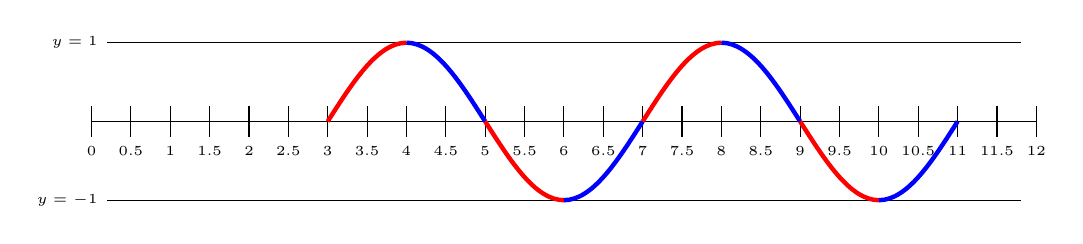
\begin{tikzpicture}

    \draw (0,0) -- (12,0);
    \draw (0.2,1)node[left,font=\tiny] {$y=1$} -- (11.8,1);
    \draw (0.2,-1)node[left,font=\tiny] {$y=-1$} -- (11.8,-1); 
    \foreach \x in {0,0.5,...,12}{
    \draw (\x,-0.2)node [below,font=\tiny,] {\x} -- (\x,0.2) ;
    }
    \draw[ultra thick, red] (3,0) sin (4,1);    %% the real business in this line
    \draw[ultra thick, blue] (4,1) cos (5,0);    %% the real business in this line
    \draw[ultra thick, red] (5,0) sin (6,-1);    %% the real business in this line
    \draw[ultra thick, blue] (6,-1) cos (7,0);    %% the real business in this line
    \draw[ultra thick, red] (7,0)  sin (8,1);    %% the real business in this line
    \draw[ultra thick, blue] (8,1) cos (9,0);    %% the real business in this line
    \draw[ultra thick, red] (9,0) sin (10,-1);    %% the real business in this line
    \draw[ultra thick, blue] (10,-1) cos (11,0);    %% the real business in this line
\end{tikzpicture}
	\caption{Veranschaulichung der Stehenden Welle im Resonanzrohr mit Wellenparametern}
	\label{ab:auswertung->Wellenlaenge->begruendung}
\end{abbildung}
Aus der Abbildung lässt sich folgender Zusammenhang ableiten:
\begin{align}
\lambda_n &= \frac{\Delta l_n}{n-1}\cdot 2
\end{align}
Mit dem Mittelwert aus \ref{sub:auswertung->MittelwertResonanzabstand} und der Gleichung wurden für jede der vier Messung die Wellenlänge $\lambda$ berechnet und in Tabelle \ref{tab:auswertung->Wellenlaenge->Ergebnis} dargestellt.
\begin{tabelle}
	\caption{Berechnete Wellenlänge für die vier Messungen}
	\label{tab:auswertung->Wellenlaenge->Ergebnis}
	\sisetup{round-precision=2}
	\begin{tabular}{|c|c|c|}
		\hline \rowcolor{firstcsvrow}
		Messung & $\overline{\Delta l_n}/cm$ & $\lambda/cm$ \\
		\csvreader[separator=semicolon, late after line = \\\hline]{./tables/Ergebnisse.csv}{}{
			\csvcoli & $\num{\csvcolvi}$ & $\num{\csvcolvii}$
		}
	\end{tabular}
\end{tabelle}

\subsection{Berechnung der Schallgeschwindigkeit $c$}
\label{sub:auswertung->Schallgeschwindigkeit}


\subsection{Korrektur des Temperatureinflusses}
\label{sub:auswertung->Temperatur}


\subsection{Zusammenfassung der Ergebnisse und Vergleich mit Literaturwert}
\label{sub:auswertung->Zusammenfassung}
%========Marius=================